% !TEX root = ../../username.tex
\section{Convolutional Neural Network} \label{sec:cnn}

\textbf{Convolutional Neural Network} (CNN) is a type of feedforward neural network designed to process images. A simple structure of a CNN consists of five types of layers. These layers are the input, convolutional, pooling, fully connected, and output layers. The fully connected layer is responsible for the actual classification process. Both fully connected and output layers behave the same as in a fully connected feedforward network discussed in Section \ref{sec:feedforward_nn}. A simple CNN structure for handwritten digit classification is shown in Figure \ref{fig:simple_cnn_diagram}.

\begin{figure}[!ht]
    \centering
    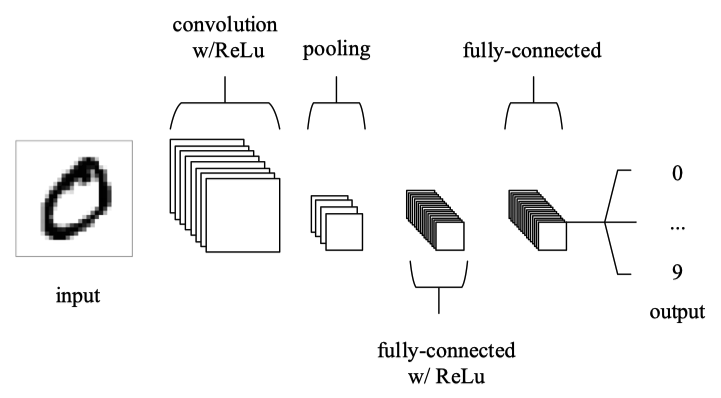
\includegraphics[width=4.5in]{figures/simple_cnn.png}
    \caption{Simple CNN structure for handwritten digit classification \cite{o2015introduction}}
    \label{fig:simple_cnn_diagram}
\end{figure}

Since an image is a 2D grid pattern data, it is possible to flatten the image and pass it through a fully connected feedforward neural network for classification directly. However, there are multiple benefits when using CNN over a standard feedforward network. The two most important benefits of CNN are spatial interaction capturing and data downsampling.

The first significant benefit is spatial interaction. \textbf{Spatial interaction} in an image refers to the connection between two or more pixel values. These connections are essential since pixels next to one another tend to describe a feature of an object, while pixels far from each other describe a different feature of the same object or a completely different object; thus, spatial interaction enhances feature extraction. On the other hand, if an image is flattened, pixels that appear close to one another will be very far away in the network, thus losing their meaning.

The second important benefit is data downsampling. \textbf{Data downsampling} refers to reducing the number of weights in the network. Consider a $64 \times 64$ RGB image, in a fully connected feedforward network, each neuron in the network will need to consider value from $64 \times 64 \times 3 = 12,288$ neurons from the previous layer. In other words, each neuron will have $12,288$ incoming connections, and the network needs to compute the gradient and do backpropagation for $12,288$ weights per neuron per network's layer. Thus, the computational and memory usage are still expensive despite the image being a low-resolution photo. Therefore, if a network could downsampling the data, it would be more efficient, have less training time, and require less computational power.

CNN is able to capture the spatial interaction and perform data downsampling using the convolutional and pooling layer before passing to a fully connected layer for classification. To further understand CNN structure, we will discuss convolutional and pooling layer functionality in detail.

\subsection{Convolutional Layer}
\textbf{Convolutional layer} is responsible for making the spatial connection and extracting features from the image. These tasks can be achieved with the use of learnable kernels. A kernel is a grid of data that has a smaller width and height but has the same depth as the input image. For example, a $64 \times 64$ RGB image will require the kernel to have the size of $x \times x \times 3$ where $x$ bounded by $2$ and $64$ inclusively. There are various types of kernels, and each type is designed to target a specific task. These tasks include blurring, sharpening, edge detection, and more. When applying the kernel to the input image, it slides from left to right and top to bottom. As it slides, the kernel's activation signal is computed by performing a scalar product of the kernel with the subregion of the image covered by it, as shown in Figure \ref{fig:kernel_op_diagram}. The kernel's activation signal represents how likely the feature -- the feature that the kernel is trying to extract -- is present at the current spatial position of the input image. The resulting grid of the kernel's activation signal is the feature map. Each kernel has an associate activation map. If multiple kernels are applied to an image, then the output feature map of these kernels will be stacked along the depth dimension.

% The kernel value are predefine for specific task. This is possible purely base on the mathematics of convolution operator. For example, a kernel with values follow the gaudience distribution, then it will give the center the kernel the highest value, and get smaller as we approach the edge of the kernel. But since the center value is effect by the value of pixels arround it, thus the sum of these make the center pixel blended in with pixels around it. Create the blurring effect.

\begin{figure}[!ht]
    \centering
    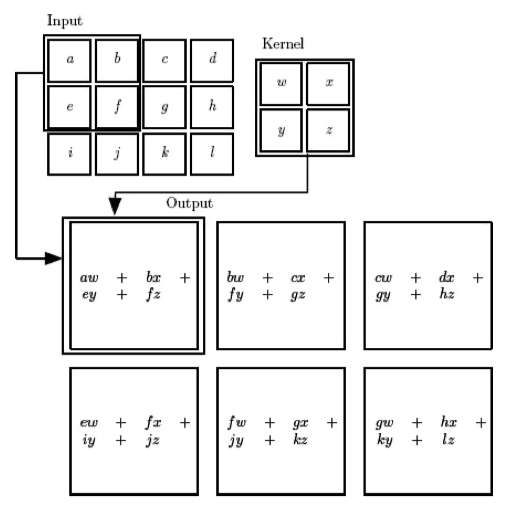
\includegraphics[width=3.5in]{figures/kernel_operation.png}
    \caption{Scalar product for a kernel's activation signal \cite{lecun2015deep}} 
    \label{fig:kernel_op_diagram}
\end{figure}
%
Notice that a kernel's width and height must be equal, and the kernel itself must be symmetric. Studies have shown that using symmetric kernels enables the algorithm to extract the inverse of a feature, thus improving the generalization for feature extraction. Additionally, since the kernel's activation signal is only based on a subregion of the image that the kernel applied to, this kernel neuron will only be connected with the neurons associated with pixels in this subregion in the network, thus reducing the number of weight in the network. The width and height of this subregion are also known as the receptive field size. Reconsider our $64 \times 64$ RGB image example, if the recaptive field is $4$, then each neuron will only have $4 \times 4 \times 3 = 48$ connections. Thus, the network will only need to compute gradient descent and do backpropagation for $48$ weights for this neuron instead of $12,288$ weights.

Other than width and height, we can also change the stride and the zero-padding to fine-tune the kernel behavior. The stride enables the kernel to slide through the image with a more significant step. That is, if the stride is 1, then the kernel will move to the left and down one pixel at a time and calculate the kernel's activation signal. Besides the stride, zero-padding also changes the convolutional behavior. The zero-padding value is the number of zero rows and columns surrounding the border of the input image. The zero-padding allows the algorithm to emphasize the border of the input image. Along with stride and zero-padding, we denoted a kernel as 
\[
    \text{kernel width} \times \text{kernel height, zero-pading size, /stride value}
\]
An the feature map size can be computed as follow:
%
\begin{equation} \label{feature_size_eq}
    \text{feature size} = \left(\frac{(\text{image size} - \text{kernel size}) + 2 \times \text{padding size}}{\text{stride}} \right) + 1
\end{equation}

\subsection{Pooling Layer}
Unlike the convolutional layer, the pooling layer only has one purpose: reducing the number of neurons in the network. The use of the pooling layer help result in fewer parameters for the network and thus require less computational power. Similar to the kernel, the pooling layer also slide through a grid of value. However, instead of sliding through the input image, the pooling layer slides through the feature map or the convoluted image to reduce the size of the feature map. There are two types of pooling layers, and they are max-pool and average-pool. As the name suggested, a max-pool layer will extract the largest activation signal in a subregion of the feature map while removing all other activation signals in the same subregion. An example of a max-pool function is shown in Figure \ref{fig:max_pool_diagram}. On the other hand, an average-pool layer takes the average value of all the activation signals in the subregion. The choice of which pooling layer to use depends on whether we care about every feature in the image equally, then the average-pool is used, or if we only care about the more prominent feature, then max-pool is used. Pooling also uses the stride to change how big of the step the pooling layer will slide through the feature map, denoted $/x$ where $x$ is stride value.
%
\begin{figure}[!ht]
    \centering
    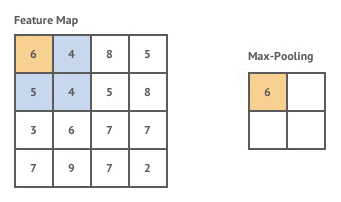
\includegraphics[width=3.5in]{figures/max_pool.png}
    \caption{$2 \times 2,\ /2$ max-pool on \cite{zeiler2014visualizing}}
    \label{fig:max_pool_diagram}
\end{figure}
%
Since pooling layer also slide throught a grid of value and output exactly one value for the subregion, thus a similar function to Equation \ref{feature_size_eq} is used to calculate the output size for pooling layer. The output size can be calculate as follow:
\[
    \text{pooling's output size} = \left(\frac{(\text{feature size} - \text{pooling size})}{\text{stride}} \right) + 1
\]

As an example, reconsider our $64 \times 64$ RGB image example, by applying a $4 \times 4, 0, \ /1$ kernel and a $2 \times 2,\ /2$ max-pool layer, the convoluted image size before passing to fully connected layer for classification is:
\[
    \text{output size} = \left[ \left( \frac{(64 - 4) + 2 \times 0}{1} + 1 \right) - 2 \right] \times \frac{1}{2} + 1 = 30 
\] 
Thus, the algorithm able to reduce from $12,288$ weights to $30 \times 30 \times 3 = 2700$ weights. In practice, it is common to have more than one kernel and one ouput apply to an input image.

% \hl{note}
% - what does NN do?
% - who came up with the idea (1-2 sentences)
% - basic des of NN archietecture
% - what is limitation of NN

% Therefore, the kernel able to perform feature extraction with spatial
% connection and reduce the number of connection per neuron.